
\section{Theoretische Grundlagen}\label{Theoretische Grundlagen}


\subsection{Neuronale Netze}\label{Neuronale Netze}

Künstliche Neuronale Netze kurz KNNs sind der menschliche
Versuch das biologische Nervensystem nachzuahmen.
Sie basieren auf der Tatsache der Reizweitergabe. 
So wird ein Eingangsreiz von Rezeptoren aufgenommen 
und über verschiedene sogenannter Neuronen weitergegeben.
Durch diese Weitergabe wird das Signal verändert,
bis ein Ausgangssignal interpretiert werden kann. 
Diese Funktionsweise macht man sich bei künstlichen
Neuronalen Netzen zu nutze.
Der Eingangsreiz sind hier 
die sogenannten \grqq features\grqq{}, 
der Ausgangsreiz eine Klasse oder ein Wert
der interpretiert werden kann.
Wir wollen uns hier nun nur auf die \grqq Feed Forward\grqq{}
Netze fokussieren. Das bedeutet das Neuronen ihre Ausgabe
nur in eine Richtung schicken dürfen.


\begin{center}
 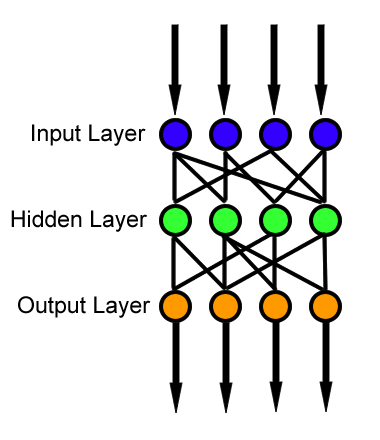
\includegraphics[width=0.4\textwidth]{abb/Feed_forward_neural_net.png}
 \captionof{figure}{Beispiel eines Feed Forward KNNs}
\end{center}


KNNs existieren in zwei Zuständen der Trainingsphase
und der Arbeitsphase. 
Die Trainingsphase ist die interessantere und wird in
dieser Arbeit beleuchtet. Hier werden durch Optimierung 
der Fehlerfunktion die Neuronen so "eingestellt" ,
dass sie einen möglichst gute Vorhersage treffen. 

Im Folgenden soll nun der Begriff des Neurons formalisiert 
werden, um die Verbesserungsmöglichkeiten des Gradienten
Verfahrens in Abschnitt \ref{Optimierungsmethoden} 
nachvollziehen zu können.

\begin{definition}
\cite[Kapitel 1.2]{BurkhardLenze.1997} Ein (\textbf{formales) Neuron} ist eine Funktion $\kappa: \mathbb{R}^n \rightarrow \mathbb{R}^m$ definiert durch:
\begin{itemize}
\item eine Aktivierungsfunktion $T:\mathbb{R} \rightarrow \mathbb{R}$
\item ein gewichteter Vektor $\vec{w} = \{w_1,w_2,...,w_n\}$
\item und eine Schwelle  $\Theta\in\mathbb{R}$.
\end{itemize}
Der Vektor $\vec{x} = (x_1,x_2,...,x_n)\in \mathbb{R}^n$ wird auf den Vektor $\vec{y} = (y,y,...,y)\in \mathbb{R}^m$ mit identischen Komponenten durch die folgende Rechenvorschrift abgebildet
\begin{align}
\kappa(\vec{x}):= (T(\sum\limits_{i=1}^n w_i x_i - \Theta),...,T(\sum\limits_{i=1}^n w_i x_i - \Theta))=\vec{y} \in \mathbb{R}^m
\end{align}   
\end{definition}
Hier seien ein paar Beispiele für Aktivierungsfunktionen angegeben
\begin{itemize}
\item Identität $T_I$
\begin{align*}
T(x):=x=T_I(x)
\end{align*}
\item Binary step
\begin{align*}
T(x) := \begin{cases} 0, \text{ for } x < 0 \\ 1, \text{ for } x \geq 0 \end{cases} =: T_1 (x)
\end{align*}
\item Sigmoid
\begin{align*}
T(x) := \frac{1}{1+e^{-x}} =: T_S(x)
\end{align*}
\item Tangens hyperbolicus
\begin{align*}
T(x) := \frac{1+tanh(x)}{2} =: T_H(x)
\end{align*}
\end{itemize}
Dies sind nur ein paar wenige Beispiele.
Jede Funktion $T:\mathbb{R}\rightarrow \mathbb{R}$
die $\lim\limits_{x \rightarrow -\infty}{T(x)}=0$ 
and $\lim\limits_{x \rightarrow \infty}{T(x)}=1$ erfüllt,
kann als Aktivierungsfunktion genutzt werden.

\begin{definition}
    \cite[Kapitel 2]{MichaelNielsen.Juni2019}
    Die \textbf{Fehlerfunktion} $J(\theta)$ eines Neuronalen Netzes ist eine 
    differenzierbare Funktion für die gilt:
    \begin{itemize}
        \item $J(\theta) = \frac{1}{n} \sum_x J_x$ wobei $x$ ein Eingabe Datum
        beschreibt.
        \item $J(\theta)$ lässt sich aus der Summe der Elemente des Ausgabe Vektors
        darstellen.
    \end{itemize}
\end{definition}

Die erste Eigenschaft bedeutet, dass die gesamte Fehlerfunktion 
sich auch durch die Fehlerfunkton der einzelnen Eingabe Daten darstellen lässt.
Diese Fehlerfunktion wird im nächsten Abschnitt minimiert werden, um
eine optimale Parameterbelegung der Gewichte $\vec{w}$ zu finden. 
Beispiele für eine solche Funktion wäre der 
mittlere quadratische Fehler.

\subsection{Gradient Descent}\label{Gradient Descent}

Der Gradient Descent oder zu Deutsch Gradienten Abstiegsverfahren
ist ein Weg eine Zielfunktion $J(\theta)$ parametrisiert durch $\theta \in \mathbb{R}^n$
zu minimieren. Man aktualisiert diese Parameter in Richtung des stärksten Abstiegs
der Zielfunktion $\nabla_\theta J(\theta)$. Die Lern Rate $\mu$ bestimmt
dabei die Größe der Aktualisierungsschritte. Das Verfahren folgt 
also der Richtung des Abstiegs der Oberfläche der Zielfunktion in ein Tal,
welches ein lokales Minimum
beschreibt. \cite[Kapitel 1]{Ruder.9152016} \\

Im Fall eines neuronalen Netzes ist die Zielfunktion $J(\theta)$ die
Fehlerfunktion des neuronalen Netzes. 
Wir brauchen einen solchen Algorithmus, da durch die Aktivierungsfunktion der Neuronen
wie in \ref{Neuronale Netze} beschrieben, die Fehlerfunktion nichtlinear wird und somit
die Minima sich nicht mehr analytisch berechnen lassen.
Um die Richtung des stärksten Abstiegs der Fehlerfunktion zu bestimmen, benötigen
wir den Gradienten.


\begin{definition}
    \cite{Konigsberger.2002}
    Der \textbf{Gradient} $\nabla$ der total differenzierbaren Funktion
    $f:\mathbb{R}^n \rightarrow \mathbb{R}$ im Punkt $a\in\mathbb{R}$ ist im
    Falle des Standard Skalar Produkts definiert durch:
    \begin{align}
        \nabla f := \frac{\partial f}{\partial x_{1}}\hat{e}_{1}+\cdots+\frac{\partial f}{\partial x_{n}}\hat{e}_{n}
    \end{align}
\end{definition}

In einfachen Worte gefasst, ist der Gradient die Ableitung einer mehrdimensionalen
Funktion, deren Funktionswerte man sich als Gebirge vorstellen kann.
Hierbei ist der Gradient in einen Punkt ein Vektor der in die Richtung des 
stärksten Anstiegs. \\
Um die Richtung des stärksten Abstiegs zu erhalten, welche wir beim Gradienten
Abstiegsverfahren benötigen, müssen wir nur den negativen Gradienten berechnen. \\\\
Mit diesem Wissen können wir nun den Standard gradient descent algorithmus definieren.

\begin{definition}
    \cite[Kapitel 2.1]{Ruder.9152016}
    Der sogenannte \textbf{batch gradient descent}, berechnet den Gradienten der 
    Kostenfunktion für den gesamten Datensatz. Jedes Update der Parameter ist definiert durch
    \begin{align}
        \theta = \theta - \eta \cdot \nabla_\theta J(\theta)
    \end{align}
    wobei $\eta$ die Lern Geschwindigkeit beschreibt.
\end{definition}


Als Algorithmus würde der batch gradient descent folgendermaßen aussehen.

\begin{lstlisting}[language=Python]
for i in range(nb_epochs ):
    params_grad = evaluate_gradient(loss_function , data , params)
    params = params  - learning_rate * params_grad
\end{lstlisting}

wobei \texttt{nb\_epochs} die Anzahl der Iterationen beschreibt. 
Diese Implementierung beschreibt die grundsätzliche Idee aber hat mehrere 
Nachteile. Da wir den Gradienten für den gesamten Datensatz berechnen ist 
diese Methode sehr langsam und nicht möglich für Datensätze, die nicht in den 
Arbeitsspeicher passen. Außerdem konvergiert dieser Algorithmus nur sehr langsam gegen
ein lokales Minimum. Zusätzlich ist die Wahl der perfekten Lern Geschwindigkeit oft
schwierig. \\

Zusätzlich benötigt man den Backpropagation Algorithmus um dieses Verfahren auf
ein gesamtes neuronales Netz anzuwenden. Dieser ist aber ebenfalls sehr komplex
und wird deshalb hier nicht behandelt. Er kann in \cite[Kapitel 2]{MichaelNielsen.Juni2019}
nachgelesen werden.

\subsection{Optimierungsmethoden}\label{Optimierungsmethoden}

Im vorherigen Abschnitt haben wir die Grundlagen des Gradienten Abstiegsverfahren
kennengelernt und gesehen, dass dieses Probleme mit sich bringt. Die folgenden
Optimierungsmethoden verbessern das grundsätzliche batch gradient descent Verfahren
in die ein oder andere Richtung.


\subsubsection{Stochastic Gradient Descent}\label{Stochastic Gradient Descent}

\begin{definition}
    \cite[Kapitel 2.2]{Ruder.9152016}
    Der Aktualisierungsschritt des \textbf{stochastic gradient descent} ist definiert durch 
    \begin{align}
        \theta = \theta - \eta \cdot \nabla_\theta J(\theta;x^{(i)};y^{(i)})
    \end{align}
\end{definition}

Der Unterschied zum \textbf{batch gradient descent} ist nur, dass der Aktualisierungsschritt
für jedes einzelne Datum ausgeführt wird. Das macht den 
Algorithmus wesentlich schneller, aber lässt ihn ebenfalls 
stärker schwanken, während er ein lokales Minimum sucht. Dies kann
positiv wie negativ sein, da eine solche Schwankung 
den Algorithmus Ebenen schneller überwinden lässt, aber manchmal
auch Minima überspringen lässt. Um eine gut Konvergenz zu gewährleisten,
erweitert man den Algorithmus noch um zwei Eigenschaften.

\begin{itemize}
    \item Die $x^{(i)}, y^{(y)}$ werden jede Iteration zufällig angeordnet
    \item Die Lern Geschwindigkeit $\eta$ wird linear verkleinert. 
\end{itemize}

Der stochastic gradient descent kann durch folgende Eigenschaft noch 
erweitert werden.

\begin{align}
    \theta = \theta - \eta \cdot \nabla_\theta J(\theta;x^{(i:i+n)};y^{(i:i+n)})
\end{align}

Nun wird nicht mehr für jedes einzelne Datum der Gradient berechnet, sondern
für einen Teilmenge der Größe $n$. In mancher Literatur, wird 
dieser Algorithmus noch einmal extra als \textbf{Mini-batch gradient descent} benannt.
\cite[Kapitel 2.3]{Ruder.9152016}. In den Implementierungen wird hier jedoch meist 
keine Unterscheidung mehr getroffen. \cite{FrancoisChollet.}

\subsubsection{Adagrad}\label{Adagrad}

Der Adagrad Algorithmus erweitert den Stochastic Gradient Descent noch weiter.
Bisher wurde die Lern Geschwindigkeit $\eta$ entweder konstant gelassen oder linear verkleinert.
Die Lern Geschwindigkeit hat somit keinen Bezug auf die Trainingsdaten. Hier setzt Adagrad an.
Er verändert die Lern Geschwindigkeit im Verhältnis zur Dichte des jeweiligen Parameters.

Deshalb hängt der Algorithmus diesmal auch von jedem einzelnen Elemente von $\theta$,
 bezeichnet als $\theta_i$ ab.
 
\begin{definition}
    \cite[Kapitel 4.3]{Ruder.9152016}
    Der \textbf{Adagrad} Algorithmus ist definiert durch den Aktualisierungsschritt
    \begin{align}
        \theta_{t+1,i} = \theta_{t,i} - \frac{\eta}{\sqrt{G_{t,ii}+\epsilon}} \cdot g_{t,i}
    \end{align}
    wobei $g_{t,i}$ definiert ist durch
    \begin{align}
        g_{t,i} = \nabla_{\theta_t} J(\theta_{t,i})
    \end{align}
    und $G_t \in R^{d\times d}$ ist eine diagonal Matrix, wobei die Diagonalelemente $i,i$, die 
    Summe der Quadrate der Gradienten zum zugehörigen Parameter $\theta_i$ bis zum Zeitpunkt
    t sind und $\epsilon > 0$ 
    
\end{definition}


\subsubsection{Adam}\label{Adam}